% !TEX TS-program = xelatex
% !TEX encoding = UTF-8 Unicode
% !Mode:: "TeX:UTF-8"

\documentclass{resume}
\usepackage{zh_CN-Adobefonts_external} % Simplified Chinese Support using external fonts (./fonts/zh_CN-Adobe/)
%\usepackage{zh_CN-Adobefonts_internal} % Simplified Chinese Support using system fonts
\usepackage{linespacing_fix} % disable extra space before next section
\usepackage{cite}
\usepackage{graphicx}


\begin{document}
\pagenumbering{gobble} % suppress displaying page number
\vspace*{-2cm}

\begin{minipage}[t]{0.72\textwidth}
  \vspace*{-3cm}
  \name{段睿}

  \basicInfo{\phone{(+86) 188-1044-7419}}
  \basicInfo{\email{buaadaniel@gmail.com}}
  \basicInfo{\faBriefcase\ 银行核心系统 / Java 高级开发}
\end{minipage}
\hfill
\begin{minipage}[t]{0.25\textwidth}
  \raggedleft
  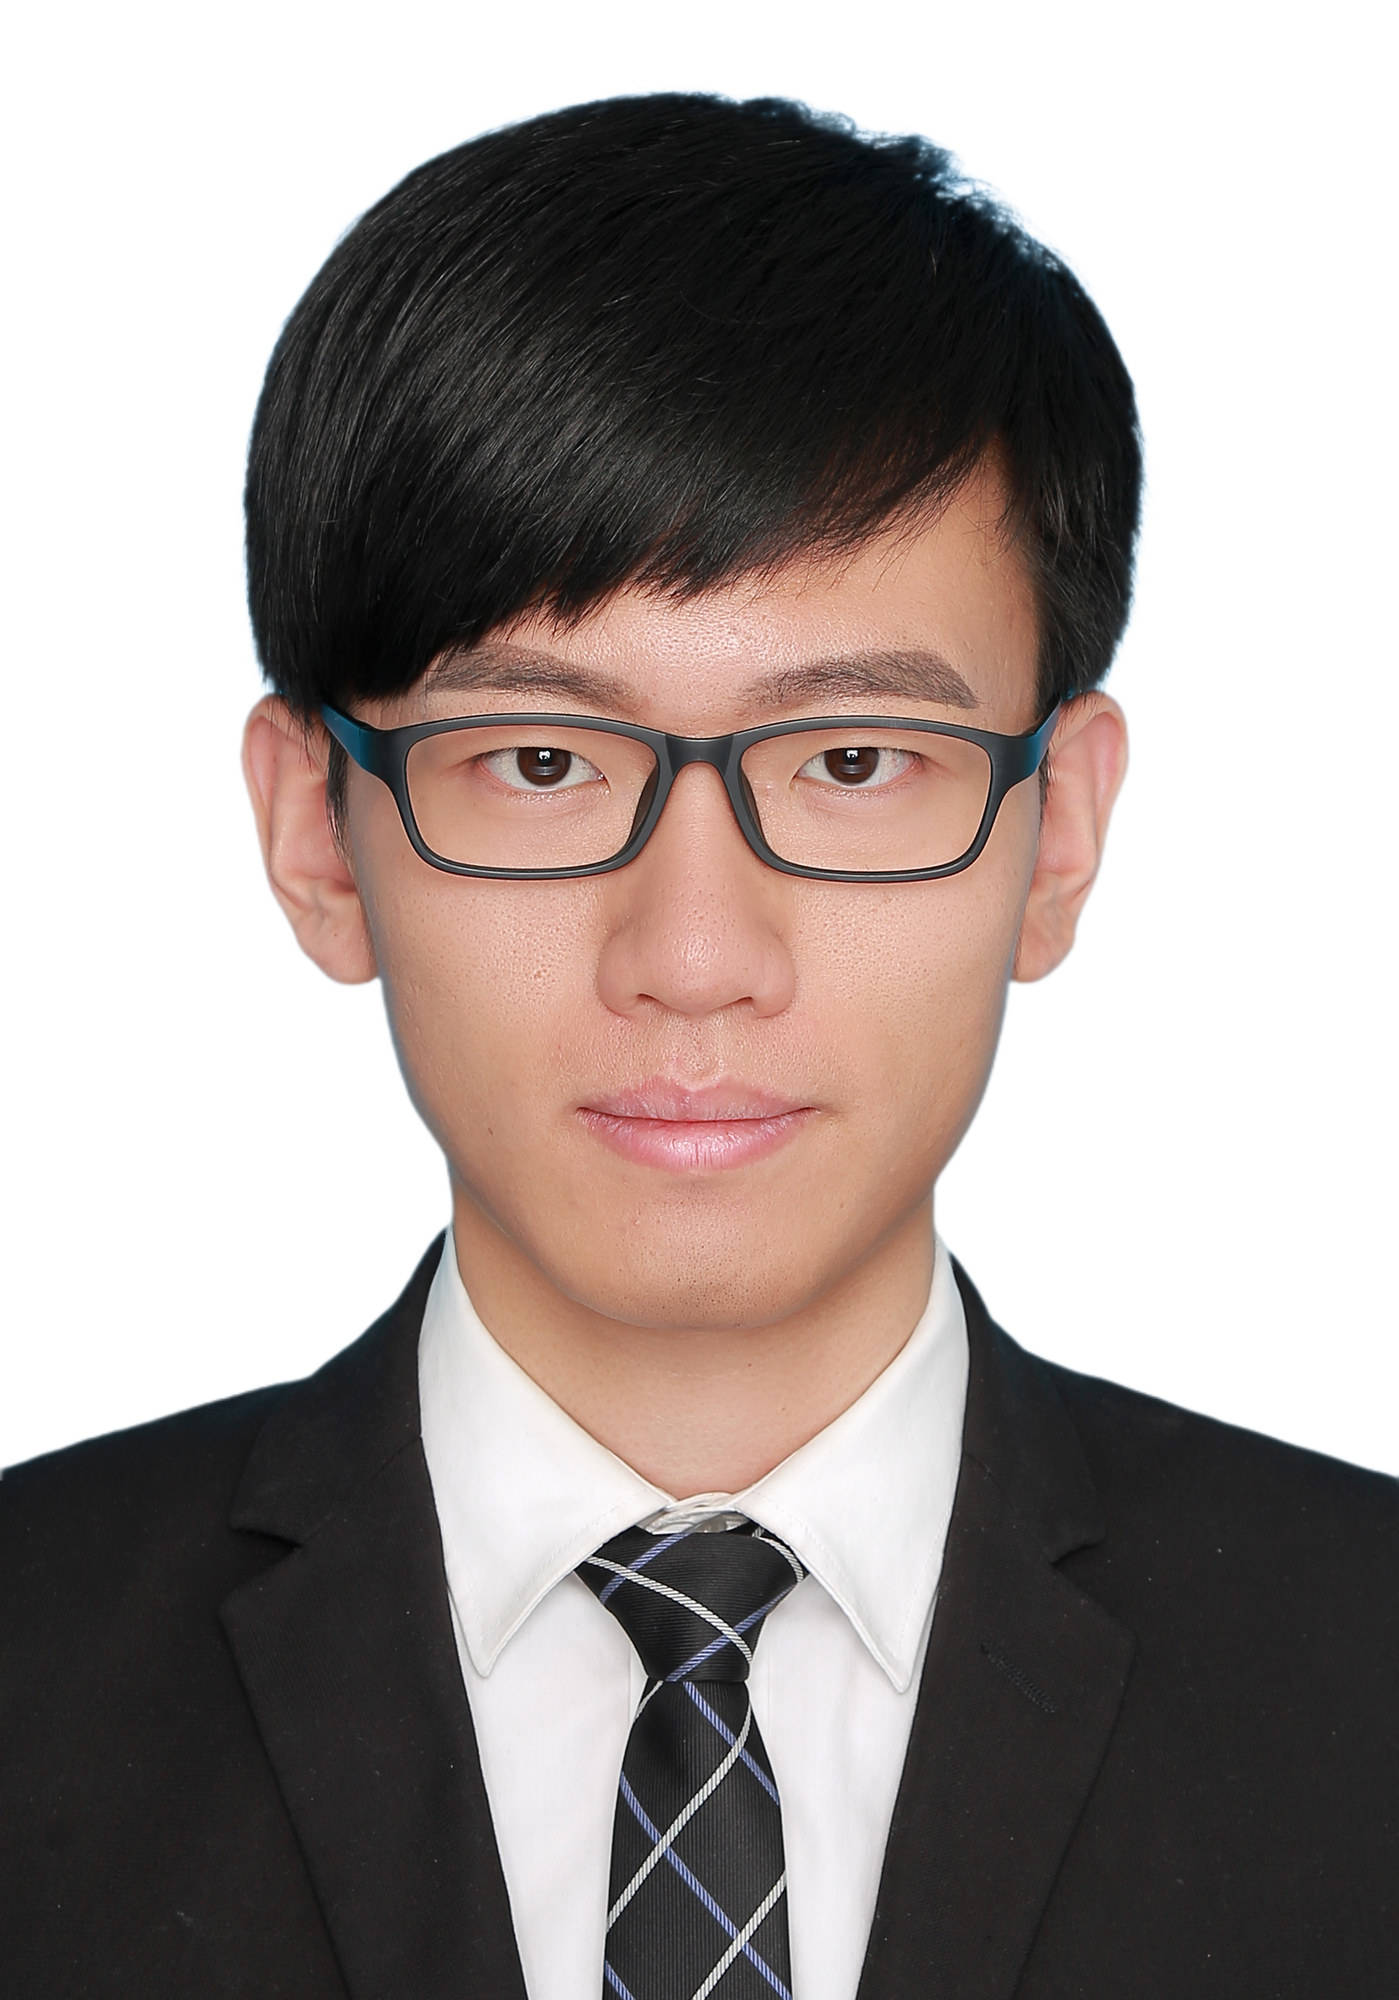
\includegraphics[width=2.8cm]{photo.jpg}
\end{minipage}

\section{\faGraduationCap\  教育背景}
\datedsubsection{\textbf{北京航空航天大学}， 北京}{2015 -- 2018}
\textit{硕士}\ 电子与通信工程-通信工程， 前20\%
\datedsubsection{\textbf{北京航空航天大学}， 北京}{2011 -- 2015}
\textit{学士}\ 电子信息工程-通信工程，前20\%

\section{\faUsers\ 工作经历}
\datedsubsection{\textbf{虾皮 -- 数字银行}， 深圳}{2021.04 至今}
\role{银行核心系统（存款、核算）Owner}{新加坡数字银行 Maribank}
\begin{onehalfspacing}
主导银行核心系统建设与演进，对账务准确性、系统稳定性及生产风险负责
\begin{itemize}
  \item \textbf{银行核心系统 Owner}：长期负责存款与核算两大核心系统，支撑日均 \textbf{40 万笔}资金交易，管理账户规模 \textbf{80 万+}，保持核心账务零重大事故
  \item 存款系统建设：设计并实现账户生命周期、记账、计结息等核心能力，引入交易幂等与重复交易拦截机制，杜绝潜在的资损风险
  \item 核算系统建设：构建标准核算输入文件系统及会计分录规则配置体系，支持年终损益结转、总账调账等关键场景，系统稳定运行近 \textbf{4 年}，核心逻辑 \textbf{0 代码变更}
  \item 存款系统迁移（进行中）：将基于神码的存款核心系统迁移至自研核心系统，负责旧系统分析改造与风险评估；通过流量重放、结果对比、可控切流等方式，实现\textbf{不停机、账务零差异}的平滑迁移
  \item \textbf{业务中心}：参与跨境汇款、行内转账等核心业务方案设计与开发；作为银行 App 业务入口服务，统一编排风控、审批、转账等流程，在保障用户体验的同时，提供\textbf{端到端账务一致性}与交易可靠性
  \item 建设\textbf{可灰度、可监控、可回滚}的发布体系（接口灰度、Prometheus/Grafana 监控），并通过性能调优保障大促期间系统稳定运行
\end{itemize}
\end{onehalfspacing}

\datedsubsection{\textbf{招银网络科技 -- 信用卡}， 深圳}{2018.05 -- 2021.03}
\role{催收系统开发}{风控开发室}
\begin{onehalfspacing}
\begin{itemize}
  \item 对原运行在S390主机、批量处理\textbf{1000万}入催案件的系统进行微服务化改造，引入\textbf{分治}并行处理模型，将批处理耗时\textbf{从5小时优化至2小时}，解决了催收客服无法按时开门作业的核心痛点
  \item 主机下移。负责主机模块功能梳理、关联分析、系统设计与实现、平滑切换
\end{itemize}
\end{onehalfspacing}

% Reference Test
%\datedsubsection{\textbf{Paper Title\cite{zaharia2012resilient}}}{May. 2015}
%An xxx optimized for xxx\cite{verma2015large}
%\begin{itemize}
%  \item main contribution
%\end{itemize}

\section{\faCogs\ 能力模型}
% increase linespacing [parsep=0.5ex]
\begin{itemize}[parsep=0.5ex]
  \item 核心能力: 分布式账务一致性、高风险系统发布治理、系统性能与容量规划
  \item 编程语言: Java, Python, Shell
  \item 技术栈: MySQL, Redis, RocketMQ, Elasticsearch, ZooKeeper, Prometheus + Grafana, Spring, Dubbo
\end{itemize}

\section{\faInfo\ 个人优势}
% increase linespacing [parsep=0.5ex]
\begin{itemize}
  \item 深度参与银行核心建设，长期担任存款与核算系统 Owner，对账务准确性与生产风险高度敏感
  \item 熟悉高风险系统的设计、上线与运维体系，具备完善的灰度、回滚与监控实践
  \item 能在复杂组织与多系统协作中推动问题落地，具备技术决策与推进能力
  \item 英语：CET-6，可进行日常技术沟通
\end{itemize}

%% Reference
%\newpage
%\bibliographystyle{IEEETran}
%\bibliography{mycite}
\end{document}
